\documentclass[10pt, a4paper]{article}

\usepackage{tar2020}

\usepackage[utf8]{inputenc}
\usepackage[pdftex]{graphicx}
\usepackage{booktabs}
\usepackage{amsmath}
\usepackage{amssymb}
\usepackage[twitter]{emoji}
\usepackage{numprint}
\usepackage{csquotes}

\DeclareMathOperator*{\argmax}{argmax}

% smile 			\emoji{1F60A}
% tired				\emoji{1F629}
% read heart		\emoji{2764}
% think 			\emoji{1F914}
% fire				\emoji{1F525}
% rolling eyes		\emoji{1F644}
% 100				\emoji{1F4AF}
% joy tears			\emoji{1F602}
% eyes				\emoji{1F440}
% blue heart		\emoji{1F499}
% two hearts		\emoji{1F495}
% crying			\emoji{1F62D}
% black heart		\emoji{1F5A4}
% stars				\emoji{2728}
% sad				\emoji{1F614}
% purple heart		\emoji{1F49C}
% skull				\emoji{1F480}
% christmas tree	\emoji{1F384}
% heart eyes		\emoji{1F60D}
	
\title{Why is emoji prediction difficult?}

\name{Matija Bertović, Antun Magdić, Ante Žužul} 

\address{
University of Zagreb, Faculty of Electrical Engineering and Computing\\
Unska 3, 10000 Zagreb, Croatia\\ 
% \texttt{autor1@xxx.hr}, \texttt{\{autor2,autor3\}@zz.com}\\
\texttt{\{matija.bertovic,antun.magdic,ante.zuzul2\}@fer.hr}
}
          
         
\abstract{
With the rise in popularity of social networks such as Facebook, Twitter, Instagram
and many others emojis have become more prominent and ubiquitous than most 
people could have expected. People today use them for various purposes and 
emojis can contain much information. Because of that they could prove to be 
useful for various NLP tasks. The same way word prediction helps models to 
"understand" words, emoji prediction could help them to "understand" emojis. 
But the task of emoji prediction is much harder than the task of predicting 
words. In this paper we compare simple models on the task of emoji prediction 
with the goal of identifying the main difficulties. We then cluster emojis to 
show main sources of problems arising in their prediction.
}

\begin{document}

\maketitleabstract

\section{Introduction}
It is not wrong to say that the world without emojis is unimaginable. Those 
miniature pictures have an enormous imapct on our lives, probably much more so than
we actually realize. Billions of emojis are used by people all around the world 
every day to better express themselves. Some use them to add emotion to the text, 
some to better communicate the message they want to send, some to indicate 
sarcasm to blur the line between written and in-person communication even more 
and some just because they like them. Sometimes emojis are used to add subtle 
details to the text, while at other times they are used to completely replace the text.
And they often replace it very well. One emoji can often contain as much, 
if not more, information as multiple words.

It is obvious that since emojis contain much information and that their understanding
could improve performance on many NLP tasks. So far, the majority of works handle 
the emoji prediction in a similar way and produced satisfying results. However, 
this problem might be too difficult the way it is currently approached. 

The task seems simple to most people because almost everyone today has an 
autocomplete keyboard that suggests emojis while the person is typing the text. 
It seems that suggestions are solid: every time one types the word \emph{sad}, 
\emoji{1F614} is suggested. But it is not very often that people really choose 
the suggested emoji. People (still) have their own minds and decide by 
themselves which emoji they want to use. There are many factors that impact the 
choice of emoji. If the model is to be successful at the task of emoji 
prediction it should understand the majority of those factors. Often, not 
all of those factors are included in the text which contains emojis.

In this paper we run two experiments. First, we compare some simple models at 
the task of emoji prediction to gain some insight about the problem. After that, 
we cluster emojis and point to some issues that should be resolved before
emoji prediction could substantially improve.

One great thing about emoji prediction is that there are much available and 
easily obtainable data. There are billions of new emojis occurrences on 
Facebook, Twitter, Instagram and various other social networks every day. In 
this paper we use data from Twitter. Ten million tweets are collected and tweets
with most frequent emojis are used for the task of emoji prediction.

\section{Related work}
Over time, emojis evolved into ubiquitous and powerful communication mechanism, especially on social networks. Therefore, there has been a rise in the number of studies trying to understand them better and even predict them. As far as we know, most of the previous works are mainly focused on emoji prediction, rather than examination of their true meaning. 

State-of-the-art results for emoji prediction task are obtained mostly by models based on bidirectional LSTMs (BLSTMs) \citep{barbieri2017}. In addition to BLSTM, attention mechanism ensures dropout of less informative words \citep{millions}. Another interesting approach to the emoji prediction problem is an investigation of the temporal information impact on emojis \citep{temporal}. It is shown that the usage of some emojis variates depending on the time of the year.

On the other hand, emoji prediction seems impossible if the meaning of emoji is unknown. \citep{mean} used skip-gram embedding model for quantitve and qualitative evaluation of Twitter emojis. Vector pair similarity and relatedness tests were performed, as well as clustering. Each emoji was represented with cluster containing most similar text tokens.

\section{Dataset}

We frame the task of emoji prediction as a supervised learning task. Each 
example is made of a tweet labelled by the emoji it contains which is removed 
from the tweet body as in \citep{barbieri2017emojis}. 

We gathered ten million tweets from the period between November 1, 2018 and 
December 31, 2018. From those tweets we extracted only the ones which contain a 
single emoji. In the final dataset we keep only the tweets where one of the 20 
most frequent emojis occurs. We split the data in train, validation and test 
sets containing \numprint{120000}, \numprint{40000} and \numprint{40000} tweets,
respectively. Classes in all sets are perfectly balanced\footnote{... as all 
things should be.}.

\section{Models and Representations}
\label{sec:models}

We experimented with various models. Different models use different input 
representations which include binary bag of words vectors, TF-IDF vectors 
\citep{manning2008introduction}, as well as100 dimensional GloVe word embeddings
pretrained on Twitter data \citep{pennington2014glove}.

In the following subsections $\hat{y}$ is used to denote the predicted class, 
and $\mathcal{Y}$ is used to denote the set of all classes. The classes are 
labelled by integers ranging from $1$ to $20$, so $\mathcal{Y} = \{1, 2, 3,
\ldots, 20\}$.

\subsection{Na\"{i}ve Bayes}

Na\"{i}ve Bayes \citep{manning2008introduction} is a probabillistic model for 
classification. It takes advantage of the Bayes rule to compute the probability 
$$P(y|\mathbf{x}) = \frac{\mathcal{L}(y|\mathbf{x}) P(y)}{P(\mathbf{x})},$$
where $y$ is the class label, $\mathbf{x}$ is the example to be classified and 
$\mathcal{L}$ is the likelihood function. Example is then assigned to the class 
$\hat{y}$ with the highest probability:

$$\hat{y} = \argmax_{y \in \mathcal{Y}} P(y|\mathbf{x}).$$

When using this model, we represent each tweet with a binary bag of words vector
and we use multivariate Bernoulli distribution as the likelihood function, where
we make the na\"{i}ve assumption of conditional independence of words in a 
tweet, given the tweet's class label.

\subsection{Logistic regression}

Logistic regression \citep{murphy2012machine} is a simple discriminative model.
We train a logistic regression classifier for each class. The output of the 
classifier trained for the class $y$ is the predicted probability that the given
example belongs to the class $y$. The probability is given by
$$P(y|\mathbf{x}) = \frac{1}{1 + e^{-(\mathbf{w}^\top \mathbf{x} + b)}},$$
where $\mathbf{w}$ and $b$ are learned parameters. We then use OVR strategy 
\citep{bishop2006pattern} to make the final classification. Class with the 
maximum predicted probability is assigned to the input example, that is 
$$\hat{y} = \argmax_{y \in \mathcal{Y}} P(y|\mathbf{x}).$$

We use this model with two different input representations: TF-IDF vectors and 
mean vectors of GloVe word embeddings of all the words in the tweet. In both 
cases we set the regularization parameter to $0.1$.

\subsection{Feed forward neural network}

Neural networks have shown to be strong performers at solving various problems,
so we also use them for the task of emoji prediction. 

We train two feed forward neural networks. One uses TF-IDF vector of a tweet as 
the input representation, while the other uses the mean vector of GloVe word 
embeddings of all the words in the tweet.

We use one hidden layer with size 100 in the network with TF-IDF input 
representation and we use three hidden layers with sizes 150, 100, 50 in the 
network with mean GloVe input representation. We set the regularization 
parameter to $10^{-5}$ for both networks.

\subsection{Bidirectional LSTM}

A class of neural networks that performs remarkably well on NLP tasks are 
recurrent neural networks. Hence, we also use a Long Short-Term Memory (LSTM) 
network \citep{hochreiter1997long}.

LSTM is a type of recurrent neural network that is able to capture long-term 
dependencies. Fully-connected layer is added after the LSTM cell to map the 
output of the LSTM cell to the vector of class logits. The final output of the 
network, i.\,e. the predicted class $\hat{y}$, is the class with the highest 
logit value:
$$\hat{y} = \argmax_{y \in \mathcal{Y}} 
    \,(\mathbf{W} \mathbf{o} + \mathbf{b})_y,$$
where $\mathbf{o}$ is the output of the LSTM cell and $\mathbf{W}$ and 
$\mathbf{b}$ are learned parameters of the fully-connected layer. $y$ is used to
index the output vector of logits, so $y$ for which the highest logit is 
obtained is selected as the predicted class.

Two bidirectional LSTM (BLSTM) layers with hidden state size of 300 are used in 
the LSTM cell. A single bidirectional LSTM layer is composed of two standard 
LSTM layers, where one is processing the input sequence from the first word to 
the last word and the other is going the opposite way. This way, both past and 
future context is available at every time step. Both of those layers' outputs 
are then concatenated into a single output vector of size 600. After the first 
BLSTM layer, a dropout layer with dropout probability $0.2$ is used. In the end,
a fully-connected layer with output size of 20 is used, because there are 20 
different classes.

Parameters are optimized using ADAM \citep{kingma2014adam} with the initial 
learning rate of $10^{-3}$. The model is trained for $20$ epochs over the train 
set with the batch size of $32$.

Each input tweet is represented by a sequence of GloVe word embeddings.

\section{Results}

We run two experiments. In the first experiment we compare various models and 
their performances on the task of emoji prediction and in the second we try to 
gain some insight about the use of emojis in tweets and the difficulties in 
their prediction.

\subsection{Experiment 1}

In experiment one we compare the performance of models described in Section 
\ref{sec:models}. It is important to stress out that our goal here was not to 
create a model that will achieve state-of-the-art results, but to experiment 
with different models and representations, compare them and try to understand 
the results. We also wanted to identify the difficulties of achieving high 
accuracies on this task, which is more thoroughly done in Experiment 2.

Achieved accuracies of the models are presented in Table 
\ref{tab:accuracy}. Only accuracies are shown since classes in test set are 
balanced.

\begin{table}
\caption{Accuracy of various models on test data. NB stand for Na\"ive Bayes, LR
for logistic regression, NN for feed forward neural network and BLSTM for 
bidirectional LSTM.}
\label{tab:accuracy}
\begin{center}
\begin{tabular}{lr}
\toprule
Model & Accuracy (\%) \\
\midrule
NB        & 51.15 \\
LR GloVe  & 33.78 \\
LR TF-IDF & 53.35 \\
NN GloVe  & 45.67 \\
NN TF-IDF & 51.05 \\
BLSTM     & 51.40 \\
\bottomrule
\end{tabular}
\end{center}
\end{table}

The best accuracy is obtained by logistic regression that uses TF-IDF 
representation.

We first compare the models without temporal information so BLSTM is left out 
for now and will be tackled later. It is clear from Table \ref{tab:accuracy} 
that the models which use TF-IDF representations perform better than the ones 
that use mean GloVe representations. Feed forward neural network with TF-IDF 
representations achieved 51.05\% accuracy and logistic regression with TF-IDF 
representations achieved 53.35\% accuracy, while the same models with GloVe 
representations achieved 45.67\% and 33.78\% accuracy, respectively. This is to 
be expected since TF-IDF vectors contain much more information than mean GloVe 
vectors, which are basically tweets reduced to a single word (that ideally
combines the senses of all the words in the tweet).

More interesting result is the following. Logistic regression regression with 
TF-IDF representations outperforms BLSTM by almost 2\%. BLSTM is a very powerful
model with a lot of hyperparameters, so it can be tuned to perform better than 
it did, but again it was not our goal to achieve the best possible 
accuracy\footnote{We were also constrained by the available computing power.}.
Results still show that taking into account temporal information, i.\,e. the 
exact word order when predicting emojis may not bring a lot more crucial 
information to the model. What is more important is the general information of 
the words from the tweet.

Another interesting, and for us surprising, fact is strong performance by the 
Na\"ive Bayes model. We conclude that the data doesn't strongly violate the 
na\"ive assumption. It also signals that TF-IDF representation maybe doesn't 
offer much improvement with repect to binary bag of words representation.

In Figure \ref{fig:confusion_matrix} the confusion matrix for feed forward 
neural network using TF-IDF representation is shown. Some interesting 
information can be extracted from the confusion matrix. It can be seen that the
model often confuses emojis in the following groups: \emoji{2764}, 
\emoji{1F495}; \emoji{1F62D}, \emoji{1F614}, \emoji{1F629}; \emoji{1F602},
\emoji{1F644} and \emoji{1F914}, \emoji{1F644}, \emoji{1F440}. Emojis in 
those groups convey the same meaning so it is reasonable that the model has 
trouble choosing between them. This issue will be explored in more detail in the
following section.
    
\begin{figure}
\begin{center}
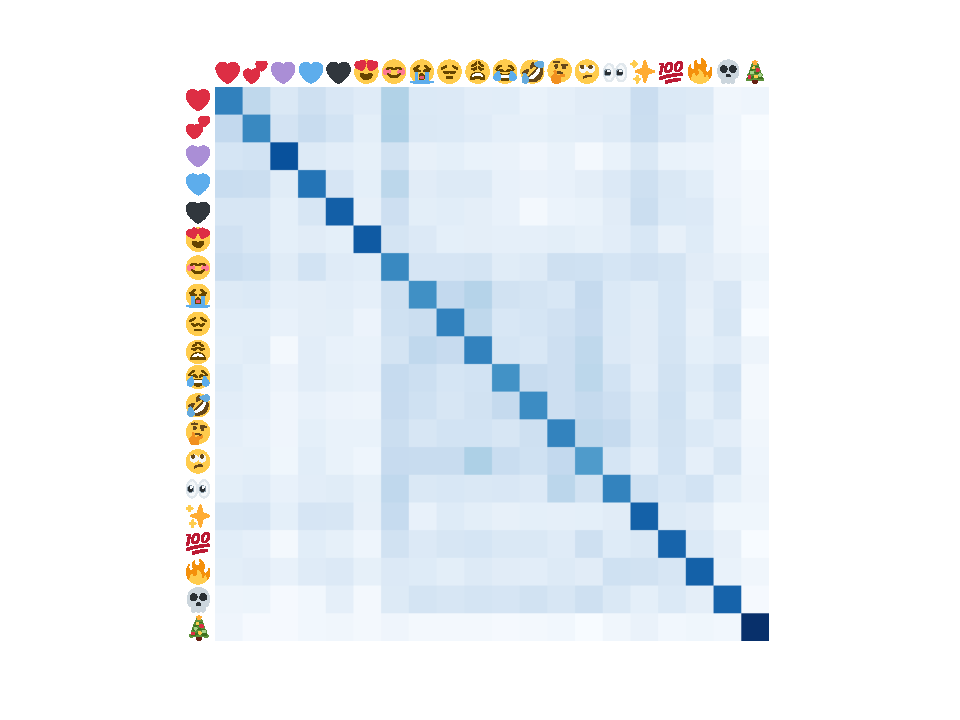
\includegraphics[width=0.8\columnwidth]{img/confusion_matrix.pdf}
\caption{Confusion matrix for feed forward neural network with TF-IDF 
representations. Values shown are square roots of real counts (for better 
visibility).}
\label{fig:confusion_matrix}
\end{center}
\end{figure}

\subsection{Experiment 2}

In the second experiment we cluster the tweets using $K$-means clustering 
\citep{bishop2006pattern}. The motivation behind this is as follows: if the 
quality of clustering is good with respect to class labels (emojis), i.\,e. 
tweets which include the same emoji are often found in the same cluster, the
task of emoji prediction is probably not very hard. On the other hand, if the 
quality of clustering is poor, the prediction is probably hard since tweets with
different emojis are not easily separable.

In this experiment we represent each tweet by the mean vector of GloVe word 
embeddings of all the words in the tweet. We believe this representation choice 
is justified by the results of the Experiment 1, where we show that temporal 
information is not crucial for emoji prediction. As can be seen from 
Table~\ref{tab:accuracy} the performance of neural network which uses mean GloVe 
vector as the input representation (model NN GloVe) achieves good enough 
accuracy compared to the models using TF-IDF vectors and sequences of GloVe word
embeddings to justify using mean GloVe vectors as representations in our 
clustering experiment, especially since the goal here isn't to develop a 
state-of-the-art method, but only to deepen the understanding of the task of 
emoji prediction.

We run the experiment for various number of classes between $20$ and $100$.
The results are qualitatively similiar in all cases. Most clusters include a 
mix of emojis without the clear winner, so we present here a few interesting and
informative examples. Clusters are shown in Figure~\ref{fig:clusters}.

\begin{figure}
\begin{center}
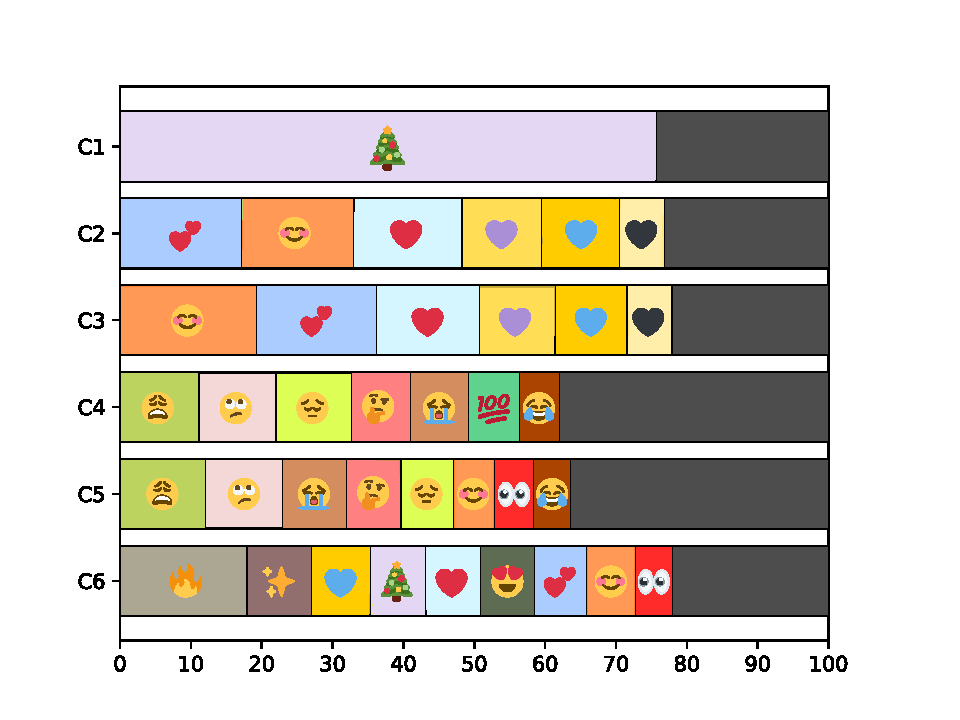
\includegraphics[width=\columnwidth]{img/clusters.pdf}
\caption{Some of the more interesting clusters. Each row represents a cluster. 
Percentages of the emojis contained in the cluster are shown on the x-axis. Only
emojis that constitute more than 5\% of the cluster are shown, while others are 
aggregated in the dark grey areas on the right side of each cluster.}
\label{fig:clusters}
\end{center}
\end{figure}

Most of the tweets in cluster C1 are Christmas themed and contain \emoji{1F384}.
They are perfect examples of tweets whose class (containing emoji) is easy to 
predict. The theme of the tweets is very clearly expressed (very often by the 
exact word \emph{Christmas}) so even the very basic models will have no trouble 
of classifying them, which can be seen easily in 
Figure~\ref{fig:confusion_matrix}. However, there are still more than 20\% of 
tweets in this cluster that don't contain \emoji{1F384}. Most of them also have 
the similar Christmassy meaning, but their authors chose a different emoji to 
accompany the message\footnote{There are also quite a few \emph{good morning} 
tweets in this cluster.}. There is no way, and it is unreasonable to expect, 
that any model might predict all of those emojis, for a model can only learn to 
assign a single emoji to a specific tweet content, but different users might 
choose different emojis. It is obvious that mere tweet content in many cases 
wont be enough to make a good prediction.

Clusters C2 and C3 show the problem of synonymy among emojis. It is obvious that
most of the tweets in those clusters convey a warm, loving, and in most cases, 
romantic message. In both clusters heart emojis make up more than 60\% of emojis
which makes it relatively easy for most models to recognize the general theme. 
But even in our limited set of 20 most frequent emojis, there are 5 heart emojis
which act as a synonyms. So even if the model is able to identify the general 
meaning of the tweet, it is still very hard for the model to predict the exact 
emoji. The reason is again that not all users will choose the same emoji to 
convey the meaning of romantic love, and without some background information 
about the author of the tweet, the model cannot make an informed decision.

Clusters C4 and C5 convey mostly negative emotions: sadness, confusion, 
annoyance and grief. It is suprising to find \emoji{1F4AF} and \emoji{1F602} in 
the mix. But the reason is pretty simple: those emojis are used here mostly in 
sarcastic setting. One could think that since thare are many sarcasm detection 
systems available, that they would be able to solve this problem. Unfortunately,
that might not be of much help because after removing the emoji most of those 
tweets don't seem sarcastic anymore, for it is the emoji that signals the 
sarcasm. With emoji removed those tweets look like all the regular tweets with 
negative sentiment, and most models would assign them the emoji accordingly. 
This could be investigated further, espacially with advances in sarcasm 
detection in mind.

Cluster C6 represents tweets with general positive sentiment that deliver joyful
messages. In most cases it is hard to pin point the emoji. For example in the 
tweet
\begin{displayquote}
I just love when we all get together!! \emoji{1F384}
\end{displayquote}
it is very hard to predict the used emoji is \emoji{1F384}. It might help if the 
model had some additional information about the tweet, like the time it was 
tweeted (which is December 25 in this example) and this was investigated in more
detail in \citep{barbieri2018exploring}. What could also help the model to 
predict the correct emoji is the picture that might accompany the tweet. If the 
example tweet included a picture of a family and a Christmas tree in the 
backgound (which is not unlikely) the problem would be much easier.

In other tweets in cluster C6 the problem of synonymy is apperent again. Some 
users might show joy and happines using \emoji{1F60A}, while others might use
\emoji{1F525} or \emoji{1F4AF}. Information about a user profile would without a
doubt be helpful in emoji prediction.

\section{Conclusion}

In this paper we investigated the difficulties that arise during the task of 
emoji prediction. Even though the task seems simple on the surface, there are 
many subtle problems that need to be solved in order to create a well performing
system for emoji prediction. We have shown that the crucial obstacle in 
achieving such a goal is synonymy among various emojis. To convey the same sense
and meaning different tweet authors choose emojis in different ways. To achieve 
better performance at emoji prediction the model would have to be fed more 
information about the user. In that way the model could identify which emoji 
from the group of synonymous emojis the author would most likely pick (based on 
his previous tweets or other information). This is a pattern that emerges in 
various NLP and AI tasks: background knowledge can be helpful and offer crucial 
information for prediction.

We don't expect that models for emoji prediction will improve substantially as 
long as information about the authors is not provided. As future work models that 
use author profiles for more informed prediction should be developed.

% \section*{Acknowledgements}

\bibliographystyle{tar2020}
\bibliography{tar2020} 

\end{document}

